\section{The Advantage Of Traces}\label{sec:advantage-traces}

Next, we present a \emph{qualitative} evaluation that compares
the explanations provided by \toolname's dynamic witnesses with
the static reports produced by the \ocaml\ compiler and \sherrloc,
a state-of-the-art fault localization approach~\cite{ZhangMyers}.
%
In particular, we illustrate, using a series of examples drawn
from student programs in the \ucsdbench\ dataset how \toolname's
jump-compressed traces can get to the heart of the error by
%
highlighting the conflicting values that cause the program to get
stuck, rather that blaming a single one,
%
showing the steps necessary to reach the stuck state, and
%
not assuming that a function is correct just because it type-checks.
%
For each example we will present
(1)~the code,
(2)~the error message returned \ocaml,
(3)~the error locations returned by \ocaml\ (underlined) and \sherrloc\ (in bold),
(4)~the jump-compressed trace produced by \toolname.

% \begin{figure*}[ht]
% \centering
% \begin{minipage}{0.49\linewidth}
% \centering


\paragraph{Example: Recursion with Bad Operator}
The recursive function @sqsum@ should square each
element of the input list and then compute the sum
of the result.
%
\begin{ecode}
  let rec sqsum xs = match xs with
    | [] -> 0
    | h::t -> ==(sqsum t)== @ (h * h)
\end{ecode}
%
Unfortunately the student has used the list-append
operator |@| instead of \texttt{+} to compute the sum.
%
Both \ocaml\ and \sherrloc\ blame the \emph{wrong location},
namely the recursive call @sqsum t@ with the message
%
\begin{verbatim}
  This expression has type
    int
  but an expression was expected of type
    'a list
\end{verbatim}
%
\toolname\ produces the following trace showing how the evaluation of
@sqsum [1]@ gets stuck:
%
\begin{center}
  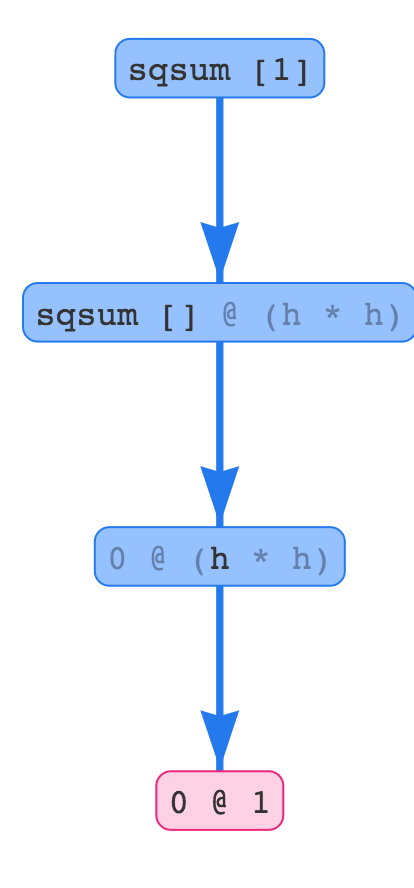
\includegraphics[height=125px]{sqsum.png}
\end{center}
%
The figure highlights the entire stuck term
(not just the recursive call), emphasizing
the \emph{conflict} between @int@ and @list@
rather than assuming one or the other is correct.

\paragraph{Example: Recursion with Bad Base Case}
%
The function @sumList@ is supposed to add up
the elements of its input list.
%
\begin{ecode}
  let rec sumList xs = match xs with
    | []    -> ==[]==
    | y::ys -> y + __sumList ys__
\end{ecode}
%
Here, the student has incorrectly returned @[]@
in the base case instead of @0@.
%
Unfortunately, \ocaml\ deduces (incorrectly)
from the base case that @sumList@ must return
a @list@, and then proceeds to blame the
\emph{recursive call} on line 3 for
producing a @list@ instead of an @int@.
%
\begin{verbatim}
  This expression has type
    'a list
  but an expression was expected of type
    int
\end{verbatim}
%
\toolname's jump compressed trace shows how the evaluation of
@sumList [1; 2]@ gets stuck when it tries to evaluate @2 + []@.
%
\begin{center}
  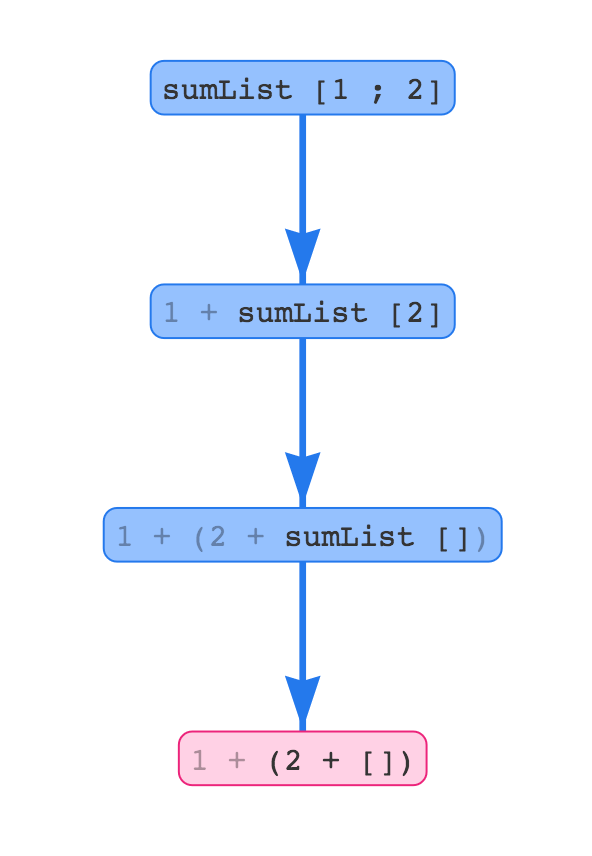
\includegraphics[height=125px]{sumlist.png}
\end{center}
%
This is essentially the same error that \ocaml produces, but the trace
clarifies immediately (via the third step) that the @[]@ is the result
of the recursive call @sumList []@, drawing attention to the incorrect
base case.

%% ES: append is actually a bit problematic as we don't find the nice
%% append [1] [2] witness. instead we could find something like
%% append [_] [], but it's not as clear IMO
% Our next example is the @append@ function, which should concatenate the
% two input lists.
% %
% \begin{ecode}
% let append xs ys = match xs with
%   | []   -> ys
%   | h::t -> h :: __t__ :: ys
% \end{ecode}
% %
% The student has forgotten to make a recursive call to @append@, and
% instead tries to cons the tail @t@ directly onto the second list @ys@.
% Consing @h@ back onto the result causes \ocaml to attempt to construct
% the infinite type @'a = 'a list@, triggering an \emph{occurs-check}
% error.
% %
% \begin{verbatim}
% Error: This expression has type
%          'a list
%        but an expression was expected of type
%          'a
%        The type variable 'a occurs inside 'a list
% \end{verbatim}
% %
% %
% \begin{center}
%   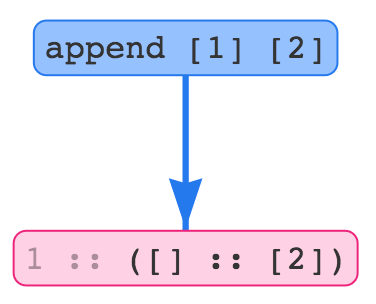
\includegraphics[height=75px]{append.png}
% \end{center}

Finally, consider the higher-order function @wwhile@ that emulates a
traditional while-loop. Concretely, @wwhile@ takes a function @f@ and
repeatedly calls @f@ on the first element of its output pair, starting
with the initial value @b@, until the second element is @false@.
%
\begin{ecode}
  let rec wwhile (f,b) =
    match f with
    | (z, false) -> z
    | (z, true)  -> wwhile (f, z)

  let f x =
    let xx = x * x in
    (xx, (xx < 100))

  let _ = wwhile (__f__, 2)
\end{ecode}
%
Unfortunately, the student has forgotten to apply @f@ at all on line 2,
and just matches it directly against a pair. This faulty definition of
@wwhile@ still typechecks however, and \ocaml thus blames the
\emph{call-site} on line 10.
%
\begin{verbatim}
  This expression has type
    int -> int * bool
  but an expression was expected of type
    'a * bool
\end{verbatim}
%
\toolname makes no assumptions about the program and quickly draws the
eye to the true error, the @match@ expression on line 2, and highlights
the conflict in matching a function against a pair pattern.
%
\begin{center}
  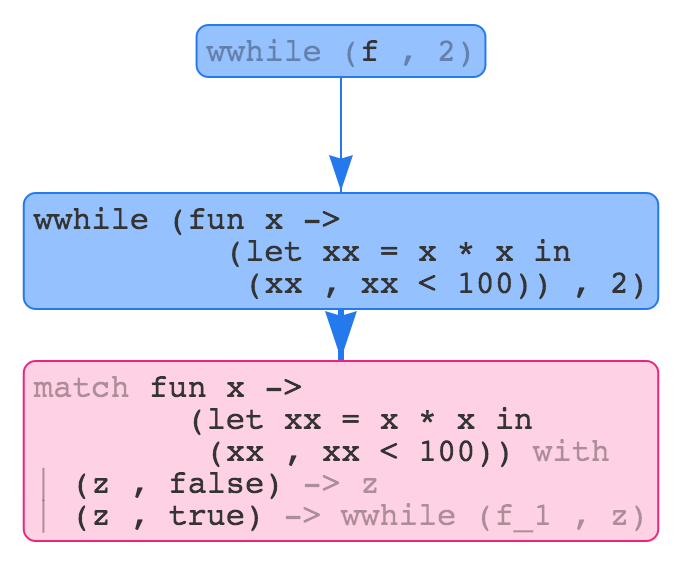
\includegraphics[height=150px]{wwhile.png}
\end{center}
%

By highlighting conflicting values rather than blaming a single value
and not making any assumptions about the given program, \toolname avoids
misleading the user into focusing their attention on a piece of code
that is actually irrelevant to the error.











%%% Local Variables:
%%% mode: latex
%%% TeX-master: "main"
%%% End:
